\subsubsection{Muon system trigger rates}
\label{sec:muontrigg}

Like the ECal, the muon system trigger rates are dominated by beam backgrounds.  
A GEANT4 model of the HPS detector was used to estimate the rates, following the conceptual design for the muon system presented in 
Section\ref{sec:muon}. Figure \ref{fig:HPS_view2} shows the layout of the system. Each of eight hodoscope layers (four layers in 
the top part of the detector and four in the bottom) consists of two planes of scintillator strips. One plane, called the Y-plane, has strips 
oriented horizontally. The other, called the X-plane, has them oriented vertically. The Y-strips are segmented exactly in the middle
and outside ends, left or right, are read out. 
Six Y-strips make up each half plane, so the total number of Y-strips is 48. 
X-planes are divided into 4.5 cm wide segments, with 240 strips in total. It should be noted that the number of vertical strips 
in the conceptual design is only 208 to limit the total number of readout channels to 256, one crate's worth. Since the rates in the 
vertical strips at the edges of the hodoscope are very low, eight strips in each 
plane can be paired to make four readout channels without negatively impacting the detector occupancy. In Table \ref{tb:muonstrp}, 
the lengths and widths of the detector readout segments (counters) used in the simulation are presented. There is a $14$ cm wide 
and $3.5$ cm high gap 
introduced into the model, centered on the point where the electron beam passes through the muon vacuum chamber, to avoid this high rate region.
As shown in Figure \ref{fig:xymu} 
this gap has a negligible effect on the detection efficiency of muon pairs from $\ap$ decays. 

\begin{table}[htdp]
\caption{Lengths and widths of the hodoscope strips. Dimensions are centimeters.}
\begin{center}
\begin{tabular}{|c|c|c|c|c|}
\hline\hline
Readout plane& Layer 1&Layer 2&Layer 3& Layer 4 \\
\hline
X-plane width& 4.5& 4.5 & 4.5 & 4.5  \\
X-plane length&10.5&11.5&12.5&13.5\\
\hline
Y-plane width& 3.5 all three&3.5, 4, 4  & 3.5, 4.5, 4.5 & 4.5 all three\\
Y-plane length&56&62.5&70&76\\
\hline\hline
\end{tabular}
\end{center}
\label{tb:muonstrp}
\end{table}%

Events generated in EGS5 were used as an input to the GEANT4 simulation. The CEBAF beam bunch structure was simulated by sending 
one bunch equivalent of electrons, 5,625 $e^-$'s (6.6 GeV), through 
the target to generate secondaries and scattered beam particles. The secondaries were followed through the apparatus
to simulate the detector response. As expected, the 
highest background rates are seen in the Layer 1 hodoscope and are $\sim 0.7$ MHz in both the X-strips near the electron beam location and 
the beam-left Y-strip closest to the beam plane, see Figure \ref{fig:l1rates}. Rates in the vertical strips far from the 
beam position are very low, allowing multiple strips to be combined into a single readout channel in order to reduce the number 
of PMTs and electronic channels.  

\begin{figure}[htbp]
\begin{center}
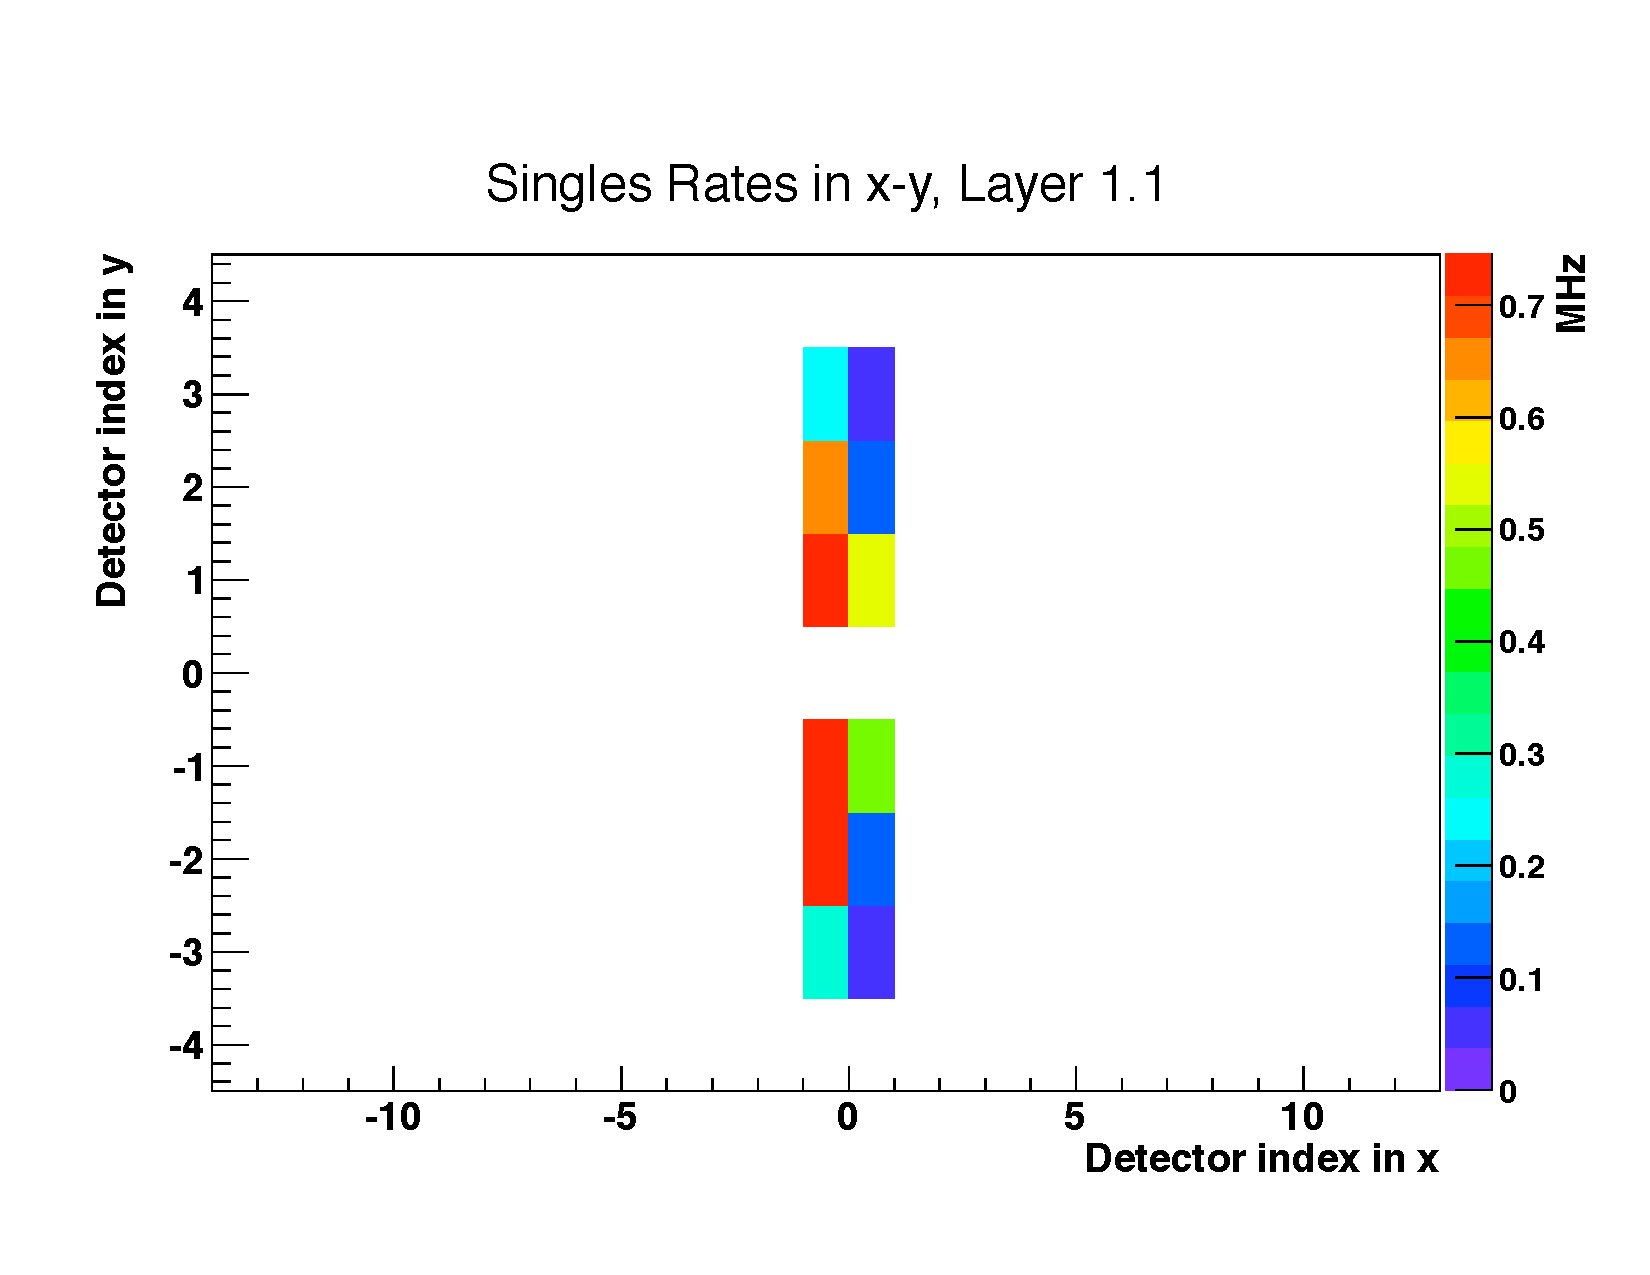
\includegraphics[width=0.475\textwidth]{performance/trigger/muon_singles1}
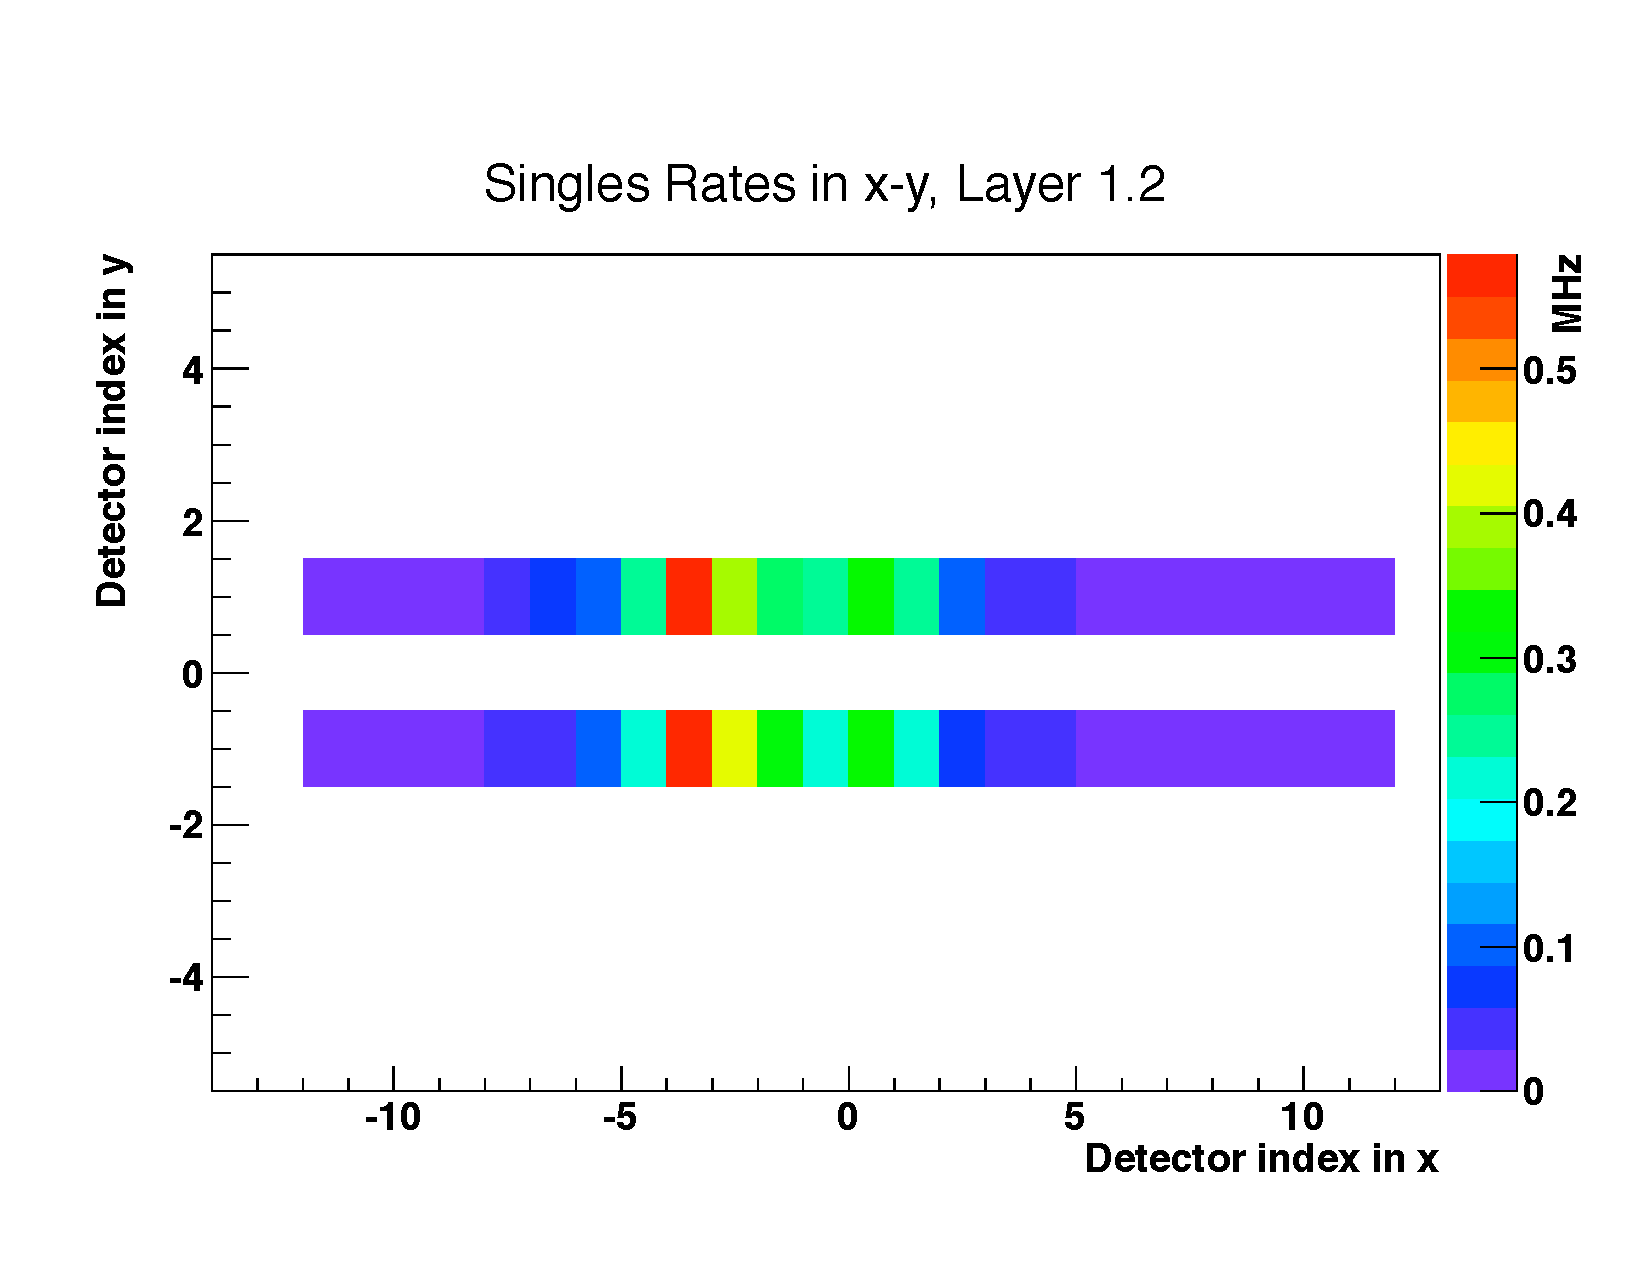
\includegraphics[width=0.475\textwidth]{performance/trigger/muon_singles2}
\caption{Rates in Y- (left) and X-planes (right) of the Layer 1 hodoscopes for hits with energy deposition $> 0.5$ MeV.}
\label{fig:l1rates}
\end{center}
\end{figure}

The coincidence rates between hodoscope planes in a given layer and between different layers have been studied using a $16$ ns coincidence 
time window. 
On the left of  Figure \ref{fig:c1rates}, the coincidence rates between X- and Y-quadrants, top-left (TL), top-right (TR), bottom-left 
(BL), and bottom-right (BR) of the Layer 1 hodoscope are shown. On the right, the figure shows coincidence rates of respective 
quadrants of Layers 1 and 2. The fact that there is a significant reduction of the rates from 2-plane (~1.2 MHz) to 2-layers (0.07MHz) 
coincidences indicates that hits are mostly from uncorrelated background. For the muon trigger, a coincidence of two opposite quadrants 
(TLxBR) or (TRxBL) is required along with triple coincidences of the first three layers of hodoscopes in each quadrant. The rates of the 
triple quadrant  
coincidences within $16$ ns are shown in Figure \ref{fig:c3rates}. The maximum trigger rates are in the beam-right (electron side) 
quadrants and are on order of $7$ kHz. In the beam-left quadrants (positron side), the tripple coincidence rates are $<1$ kHz. 
Since an overall trigger requires hits in two opposite quandrants, the maximum 
rate will be $<1$ kHz. While a further reduction of rates will be possible with the inclusion of 
MIP hits in the ECal, the $<1$ kHz is a small addition to the total trigger rate from the Ecal trigger (see discussions in 
Section \ref{sec:ecaltrigg}) and will keep overall trigger rate well within the limit of allowed rates for the HPS DAQ.   

\begin{figure}[htbp]
\begin{center}
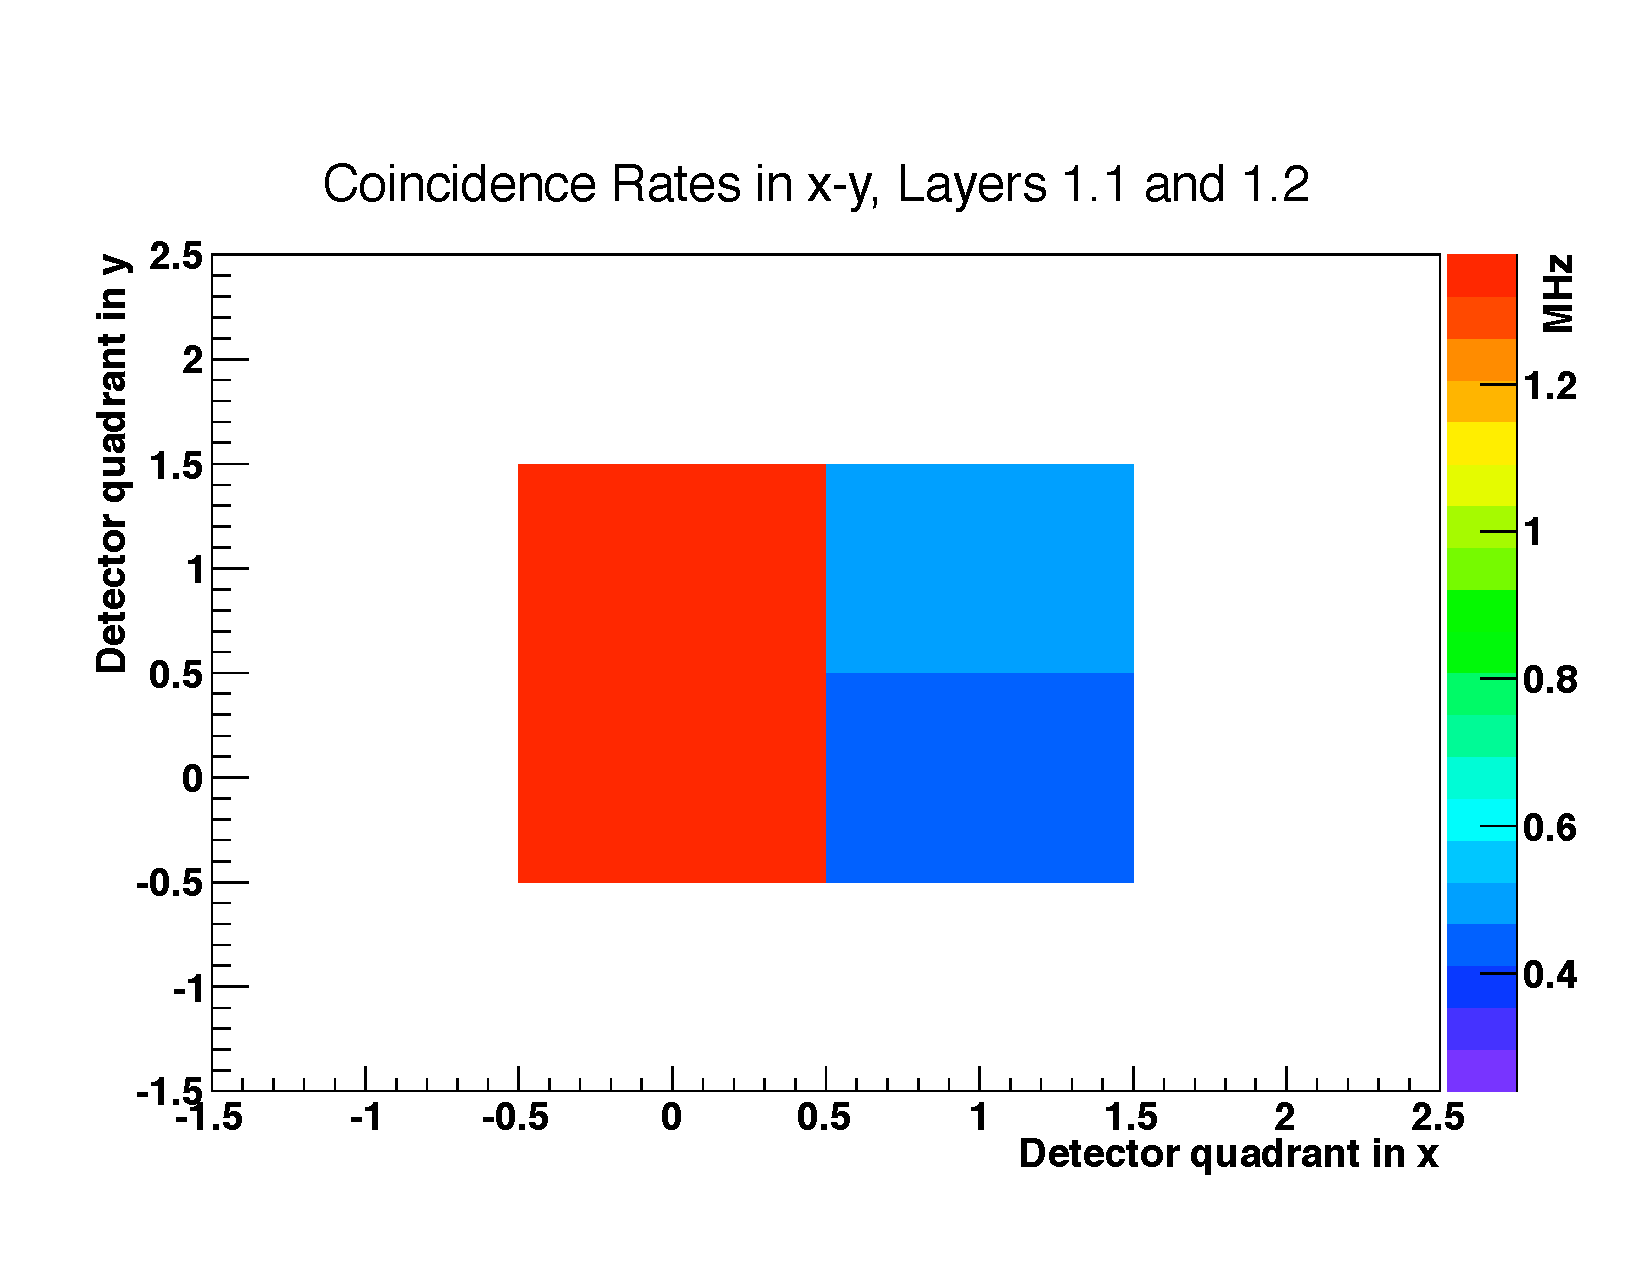
\includegraphics[width=0.475\textwidth]{performance/trigger/muon_coinrate1}
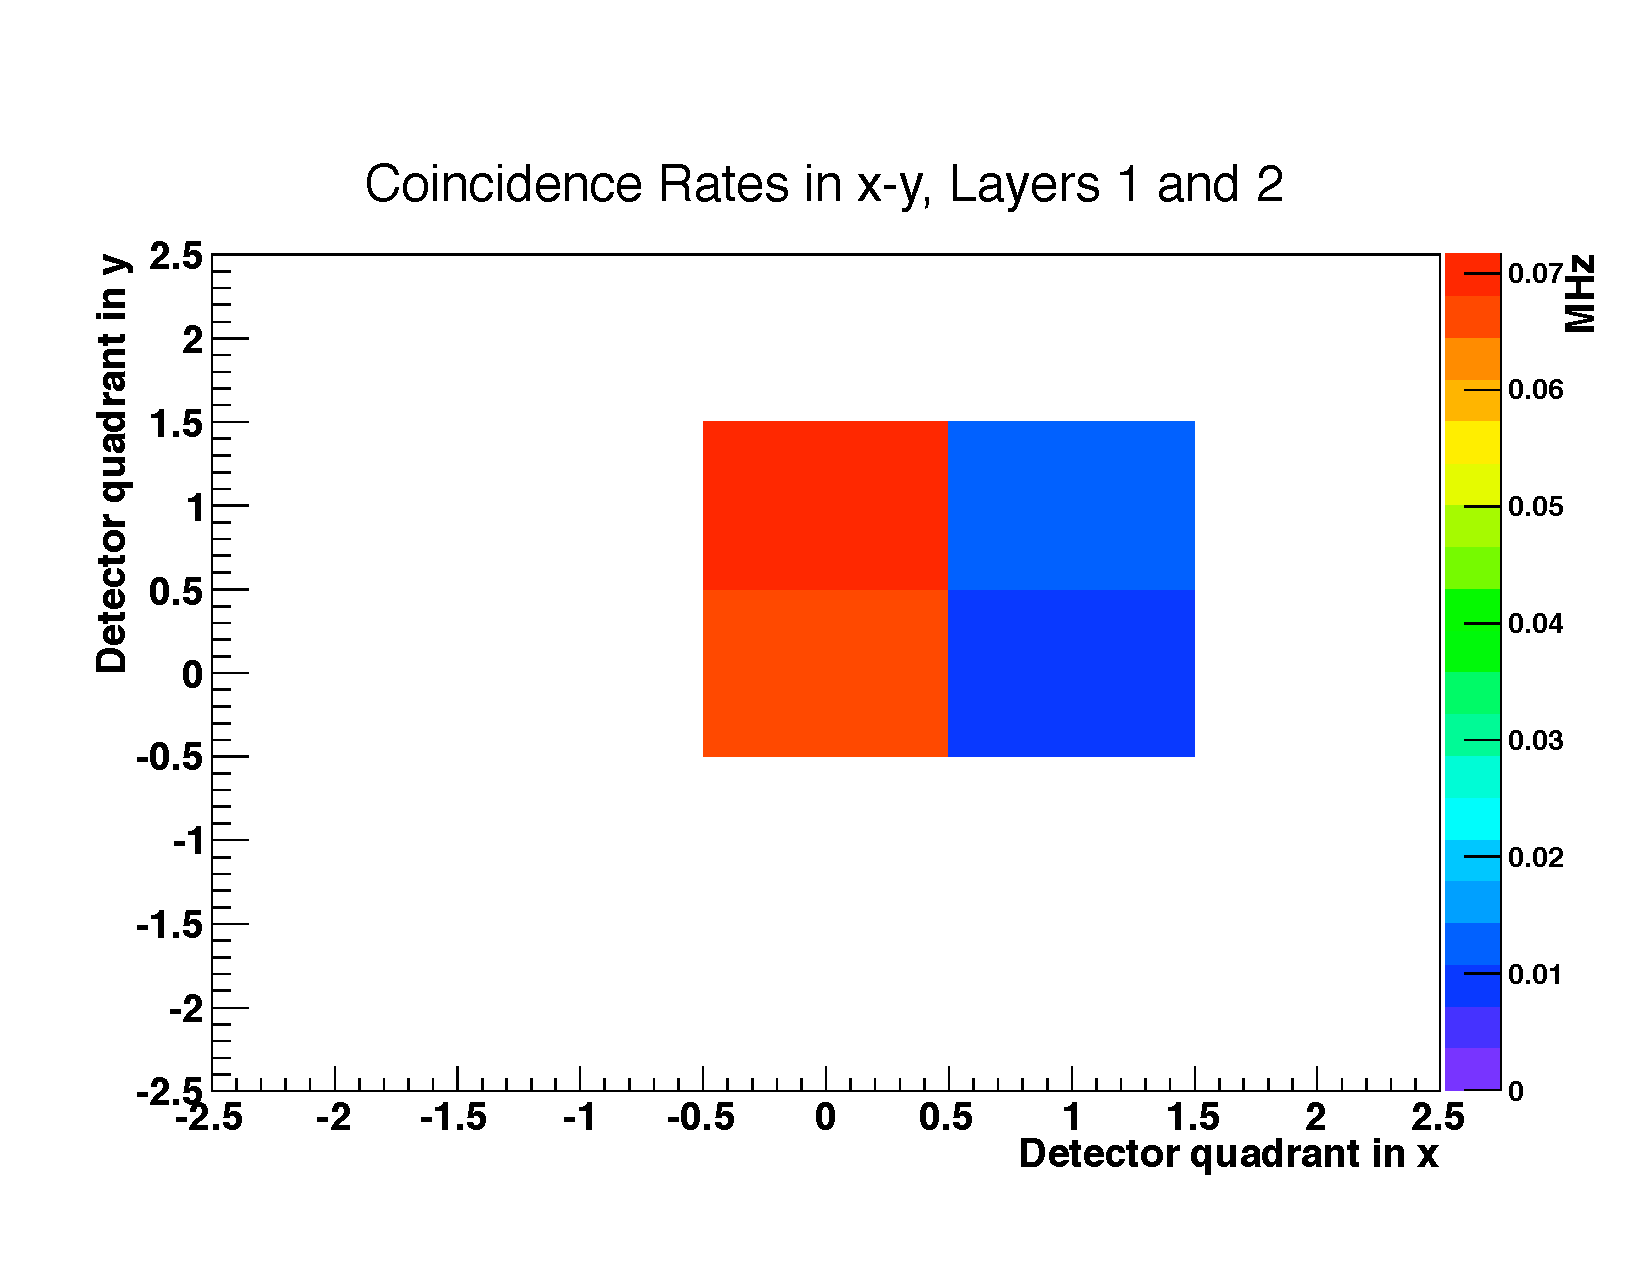
\includegraphics[width=0.475\textwidth]{performance/trigger/muon_coinrate2}
\caption{Coincidence rates between X- and Y-quadrants of the Layer 1 hodoscope (left graph) and coincidence rates between Layer 1 and 2 
(right graph). }
\label{fig:c1rates}
\end{center}
\end{figure}

\begin{figure}[htbp]
\begin{center}
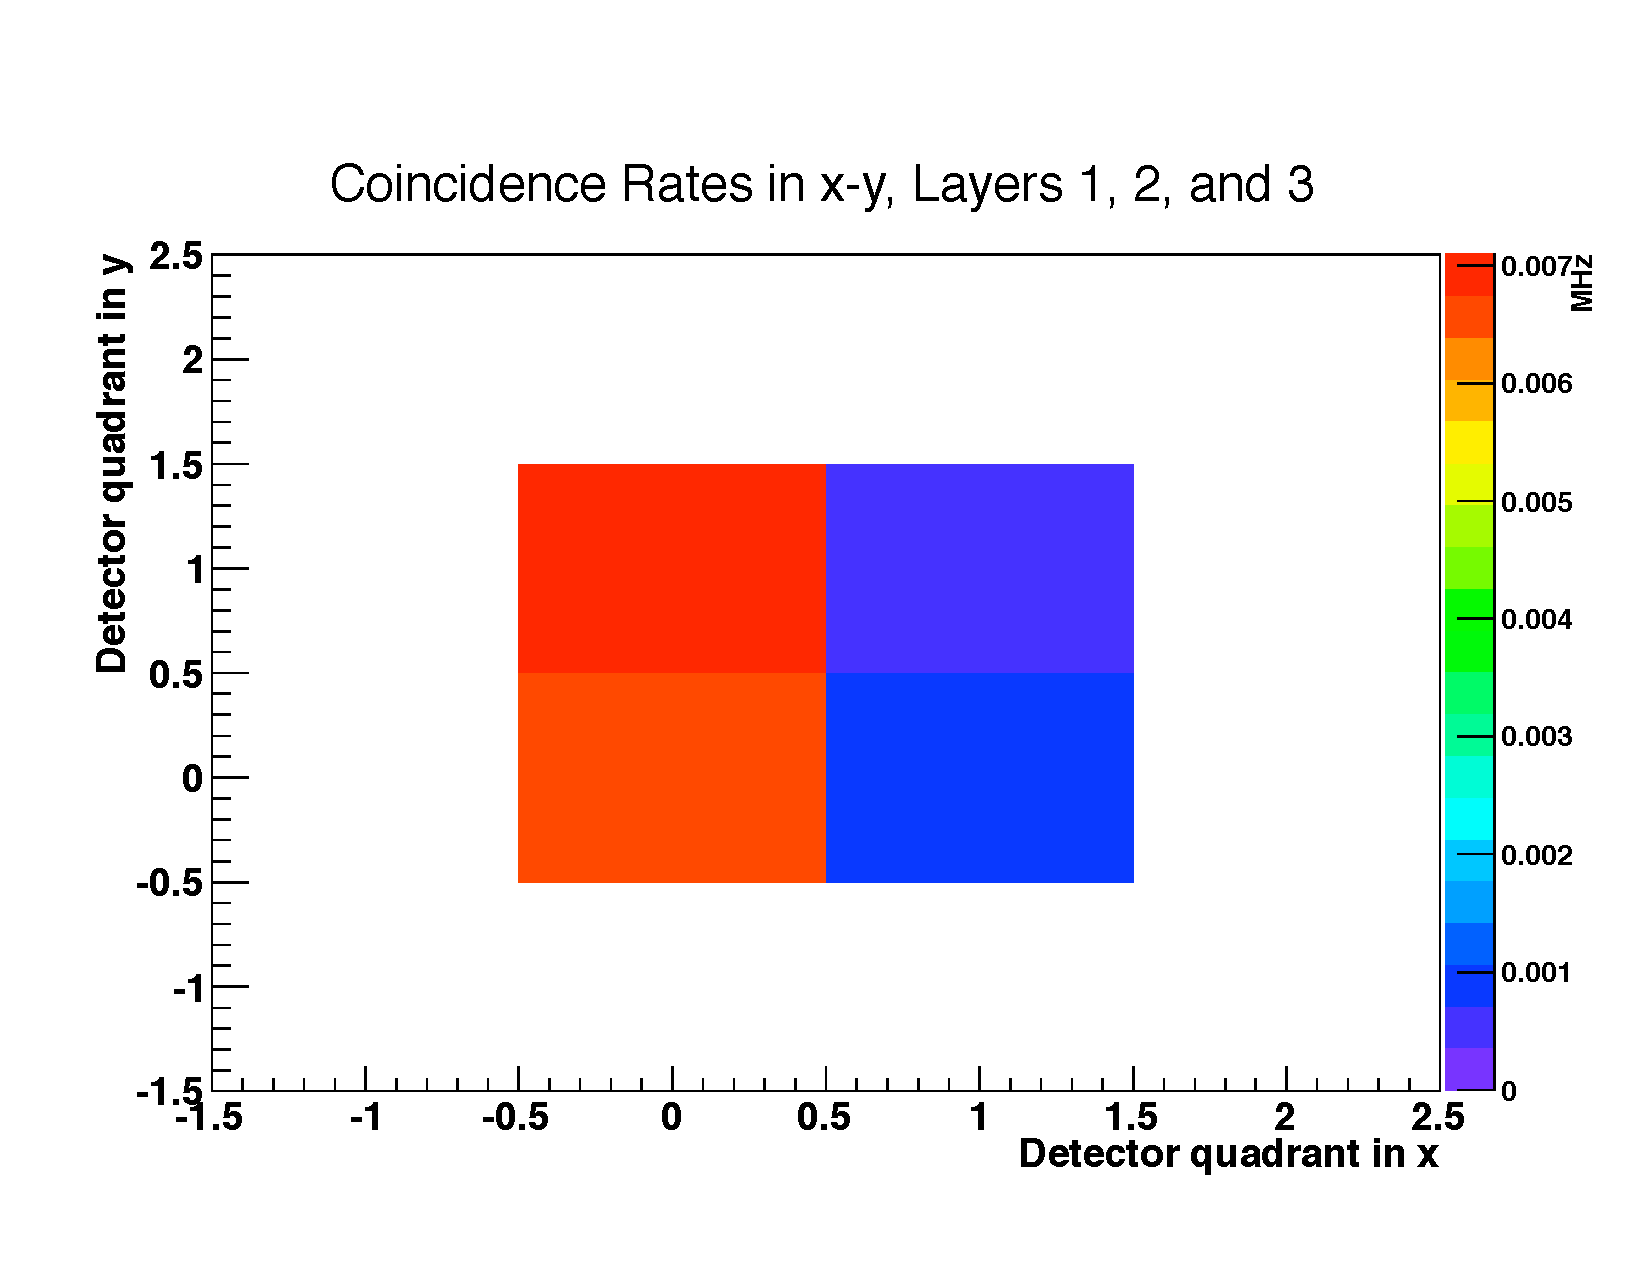
\includegraphics[width=\textwidth]{performance/trigger/muon_coinrate3}
\caption{Coincidence rates in first three layers of muon hodoscopes. The coincidence time window is set to $16$ ns. }
\label{fig:c3rates}
\end{center}
\end{figure}





